\documentclass[../main.tex]{subfiles}
% !TeX root = ../main.tex
\begin{document}
	\section{Analyzing and Recording Transactions}
	
	\subsection{Analyzing and Recording Processes}
	
	The process has the following steps:
	\begin{itemize}[noitemsep]
		\item Analyze each transaction and event from \textbf{source documents}.
		\item Record relevant transactions and events in \textbf{journal}.
		\item Post journal information to ledger accounts.
		\item Prepare and analyze trial balance.  
	\end{itemize}
	
	\subsubsection{Source documents}
	
	\textbf{Source documents} identify and describe transactions and events 
	entering the accounting process \eg checks, employee earnings records, 
	bills from suppliers, purchase orders, bank statements, sales tickets. They 
	are sources of accounting information 
	and can be in either hard copy or electronic form. 
	
	\subsection{The Account and Its Analysis}
	
	An \textbf{account} is a record of increases and decreases in a specific 
	asset, liability, equity, revenue or expense item. Information from an 
	account is analyzed, summarized and presented in reports and financial 
	statements. 
	
	The \textbf{general ledger} or \textbf{ledger}, is a record 
	containing all accounts used by a company. While most companies' ledgers 
	contain similar accounts, a company often uses one or more unique accounts 
	because of its type of operations. Accounts are classified into three 
	general categories based on the account equation \ie asset, liability or 
	equity. 
	\[
	\text{Asset Accounts} = \text{Liability Accounts} + \text{Equity Accounts}
	\]
	
	\subsubsection{Asset Accounts} 
	
	Assets are resources owned or controlled by a company and 
	that have expected future benefits. Most accounting systems include (at a 
	minimum) separate accounts for the assets \eg cash, 
	accounts receivable, note receivable, and prepaid accounts.
	\begin{itemize}[noitemsep]
		\item A \textbf{cash account} reflects a company's cash balance. It 
		includes money and any medium of exchange that a bank accepts for 
		deposit \eg coins, check.
		\item \textbf{Accounts receivable} are held by sellers and refer to 
		promises of 
		payment from customers to sellers. These transactions are often called 
		\textbf{credit sales} or \textbf{sales on account} or on 
		\textbf{credit}. Accounts Receivable are increased by credit 
		sales and decreased by customer payouts. 
		\item A \textbf{note receivable}, or promissory note, is a written 
		promise of another entity to pay a definite sum of money on a specified 
		date to the holder of the note. A company holding a promissory note 
		signed by another entity as an asset that is recorded in a \textbf{Note 
		(or Notes) Receivable}.
		\item \textbf{Prepaid Accounts} (prepayments or prepaid expenses) are 
		assets that represent prepayments of future expenses (not current 
		expenses). When the expenses are later incurred, the amounts in prepaid 
		accounts are transferred to the expense accounts. When financial 
		statements are prepared, prepaid accounts are adjusted so that 
		\begin{itemize}[noitemsep]
			\item All expired and used prepaid accounts are recorded as regular 
			expenses.
			\item All unexpired and unused prepaid accounts are recorded as 
			assets. 
		\end{itemize}
		\item \textbf{Supplies} are assets until they are used. When they are 
		used up, 
		their costs are reported as expenses. The costs of unused supplies are 
		record in the Supplies asset account. Supplies are often 
		grouped by purpose. 
		\begin{itemize}[noitemsep]
			\item Office supplies \eg stationery, paper, toner and pens
			\item Store supplies \eg packaging materials, plastic and paper. 
		\end{itemize}
		\item \textbf{Equipment} is an asset. When equipment is used and gets 
		worn down, its cost is gradually reported as an expense 
		(\textbf{depreciation}). Equipment is grouped by its purpose. \eg 
		\textbf{Office Equipment}, \textbf{Store Equipment}
		\item \textbf{Buildings} \eg stores, offices, warehouses, and 
		factories are assets because they provide expected future benefits to 
		those who control or own them. 
		\item \textbf{Land} account records the cost of land owned by a 
		business. 
	\end{itemize}
	
	\subsubsection{Liability Accounts} 
	
	\textbf{Creditors }are individuals and 
	organizations that have rights to receive payments from a company. If a 
	company fails to pay its obligations, the law gives creditors a right to 
	force the sale of that company's assets to obtain the money to meet 
	creditor's claims. When assets are sold under these conditions, creditors 
	are paid first, but only up to the amount of their claims. Any remaining 
	money goes to the owners of the company. These are some liability accounts:
	\begin{itemize}[noitemsep]
		\item \textbf{Accounts payable} refer to the oral or implied promises 
		to pay later.
		\item \textbf{Note payable} refer to a formal promise to pay a future 
		amount. 
		\item \textbf{Unearned Revenue} refer to a liability that is settled in 
		the future when a company delivers its products or services. When 
		products ar delivered, the earned portion of the unearned revenue is 
		transfered to the revenue accounts.
	\end{itemize}
	
	\subsubsection{Equity Accounts} 
	
	The owner’s claim on a company’s assets is called equity. Equity is the 
	owner’s residual interest in the assets of a business after deducting 
	liabilities.
	
	When an investor receives shares for investing in a company, 
	the invested amount is recorded in an account called \textbf{Share 
	Capital}.  Any further issuance of shares are recorded in this account. 
	Dividends are not expenses of the business and are simply the opposite of 
	share capital. 
	
	\subsection{Analyzing and Processing Transactions}
	
	The collection of all accounts and their balances for an information system 
	is called a \textbf{ledger}. A company's size and diversity of operations 
	affect the number of accounts needed.  
	
	\begin{figure}[ht]
		\centering
		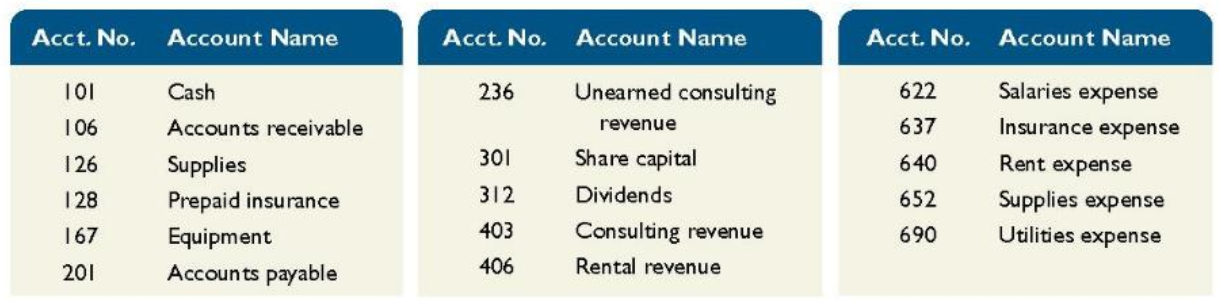
\includegraphics[width=1\columnwidth]{images/c2/chart_of_accounts.png}
		\caption{\textbf{Chart of Accounts.} Notice that all asset accounts 
		begin with a 
		prefix of one, liability accounts with two, \etc}
	\end{figure}
	
	A \textbf{chart of accounts} is a 
	list of all ledger accounts and includes an identification number assigned 
	to each account. These numbers provide a three-digit code that is useful 
	for record-keeping. 
	
	\subsubsection{Debit and Credit}
	
	A \textbf{T-account} represents a ledger account and is a tool used to 
	understand the effects of one or more transactions. The layout of a 
	T-account has the account title on the top, a left, or \textbf{debit} side 
	and a right or \textbf{credit} side.
	
	\begin{figure}[ht]
		\centering
		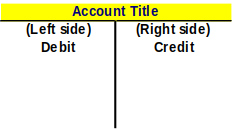
\includegraphics[width=.5\columnwidth]{images/c2/t_account.png}
		\caption{T-account}
	\end{figure}
	
	To debit an account, enter amounts on the left side of the account and to 
	credit the account, enter the amounts onto the right side. Whether a 
	debit/credit is an increase or decrease depends on the account. The 
	difference between the total debits and total credits for an account, 
	including any beginning balance is the \textbf{account balance}. When the 
	sum of debit exceeds the sum of credits, the account has a \textbf{debit 
	balance}. It has a \textbf{credit balance} when the sum of credits exceed 
	the sum of debits and a \textbf{zero balance} when the sum of credits equal 
	the sum of debits. 
	
	\subsubsection{The Debit/Credit Framework}
	
	Take special note of three important rules when updating a T-account:
	\begin{itemize}[noitemsep]
		\item Accounts increase on the same side as they appear in the 
		accounting equation $A = L + SE$ \ie accounts on the left side of the 
		accounting equation increase on the left side of the account and 
		accounts on the right side of the equation increase on the right.
		\begin{figure}[ht]
			\centering
			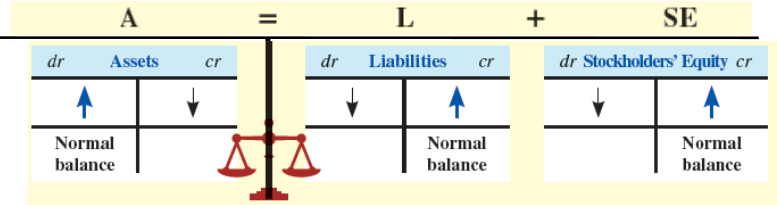
\includegraphics[width=1\columnwidth]{images/c2/debit_credit_framework.png}
			\caption{Debit/Credit Update}
		\end{figure}
		\item Left is debit (dr), right is credit (cr). 
		\begin{itemize}[noitemsep]
			\item Use debits for increases in assets (and for decreases in 
		liabilities and stockholders’ equity accounts). 
			\item Use credits for increases in liabilities and 
		stockholders’ equity accounts (and for decreases in assets).
		\end{itemize}
		\item The normal balance for an account is the side on which it 
		increases. Assets normally have debit balances, whereas liabilities and 
		stockholders’ equity accounts normally have credit balances.
	\end{itemize}
	
	This the expanded credit framework for Shareholder's Equity:
	
	\begin{figure}[ht]
		\centering
		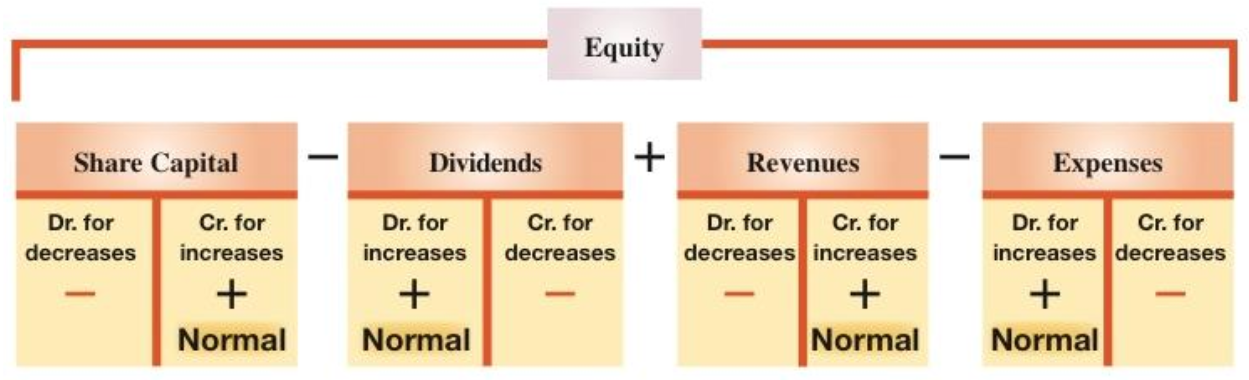
\includegraphics[width=1\columnwidth]{images/c2/expanded_framework.png}
		\caption{Expanded Shareholder's Equity for Debit/Credit}
	\end{figure}
	
	\subsubsection{Double Entry Accounting}
	
	\textbf{Double Entry Accounting} requires that for each transaction:
	\begin{itemize}[noitemsep]
		\item At least two accounts are involved, with at least one debit and 
		one credit.
		\item The total amount debited must be equal to the total amount 
		credited. 
		\item The accounting equation must not be violated. 
	\end{itemize}
	
	The sum of debits for all entries must equal the sum of credits for all 
	entries. The sum of debit account balances in the ledger must equal the sum 
	of credit account balances.  This means that a net increase in Asset 
	accounts must have a net increase in the sum of Liability and Equity 
	accounts. 
	
	\begin{figure}[ht]
		\centering
		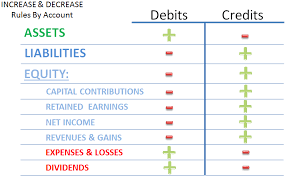
\includegraphics[width=.6\columnwidth]{images/c2/credit_debit.png}
		\caption{Accounts and normal balances}
		\label{fig:accounts}
	\end{figure}
	
	\subsection{Journalizing and Posting Transactions}
	
	A \textbf{journal} gives a complete record of each transaction in one 
	place. It also shows the debits and credits for each transaction. The 
	rpocess of recording transactions in a journal is called 
	\textbf{journalizing}. Step 4 is to transfer or post entries from journal 
	to the ledger. The process of transferring journal entry to the ledger is 
	called \textbf{posting}.
	
	\subsubsection{Journalizing Transactions} The process of journalizing 
	transactions requires an understanding of a journal. While companies can 
	use several journals, every company has a \textbf{general journal}. It can 
	be used to record any transaction and the following information about each 
	transaction:
	\begin{itemize}[noitemsep]
		\item Date of transaction
		\item Titles of affected accounts
		\item Dollar amount of each debit and credit
		\item Explanation of transaction
	\end{itemize}

	\begin{figure}[ht]
		\centering
		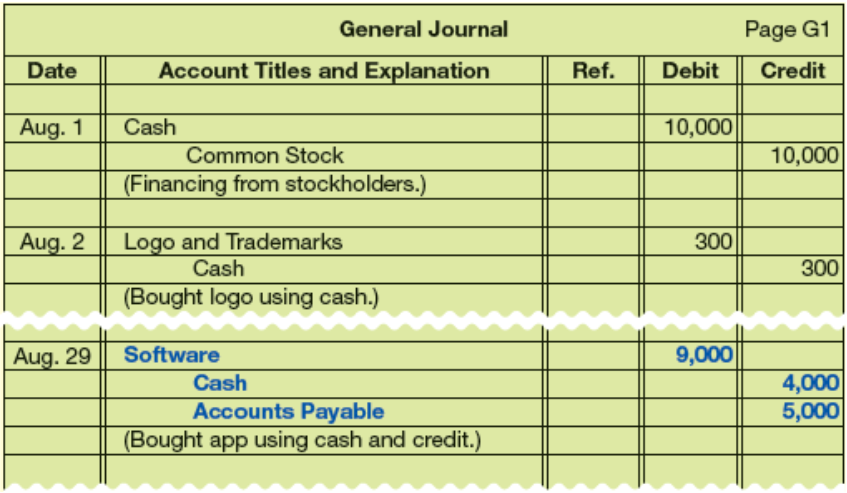
\includegraphics[width=1\columnwidth]{images/c2/general_journal.png}
		\caption{General Journal}
	\end{figure}
	

	The general journal is a chronological listing of the transactions. At the 
	end of the accounting period, we post the information from the general 
	journal to the proper general ledger account. The general ledger groups all 
	transactions that impact a particular account. That is, all the 
	transactions that increase or decrease the cash account are posted to the 
	general ledger cash account. To record entries into a journal, apply these 
	steps:
	\begin{enumerate}[noitemsep]
		\item \textbf{Date the transaction} -  Enter the year at the top of the 
		first column and the month and day on the first line of each journal 
		entry.
		\item Enter the titles of the accounts debited and then enter amounts 
		in the Debit column on the same line
		\item Enter the titles of the accounts credited and then enter amounts 
		in the Credit column on the same line. Account titles are form the 
		chart of accounts and are aligned with the left margin of the Account 
		Titles and Explanation column.
		\item Enter a brief explanation of the transaction below the entry.  
		\item A blank line is left between each journal entry for clarity. When 
		a transaction is first recorded, the \textbf{posting reference (PR) 
		column} is left blank (in a manual system). Later, when posting entries 
		to the ledger, the identification numbers of the individual ledger 
		accounts are entered in to the PR column.
	\end{enumerate}

	\begin{figure}[ht]
		\centering
		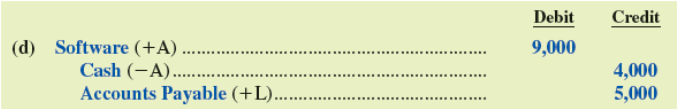
\includegraphics[width=1\columnwidth]{images/c2/simplied_journal_format.png}
		\caption{Simplified Format for General Journal}
	\end{figure}
	For classroom purposes, we use a simplified version of a journal entry 
	which should make it easier for you to learn the most important aspects of 
	recording journal entries. The main differences between the simplified 
	format and a formal journal entry are:
	\begin{itemize}[noitemsep]
		\item When a date is not given, use some form of reference for each 
		transaction, such as (d), to identify the event.
		\item Omit the reference column and transaction explanation to simplify 
		the entry.
		\item Include the appropriate account type (A, L, or SE) along with the 
		direction of the effect ( + or - ) next to each account title to 
		clarify the effects of the transaction on each account. This 
		parenthetical note will reinforce the debit/credit framework and help 
		you ensure the accounting equation remains in balance.
	\end{itemize}

	
	\subsubsection{Posting Entry to Ledger}
	
	For classroom purposes we will use a simplified format for ledger accounts 
	to make it easier to focus on their main features. 
	
	\begin{figure}[ht]
		\centering
		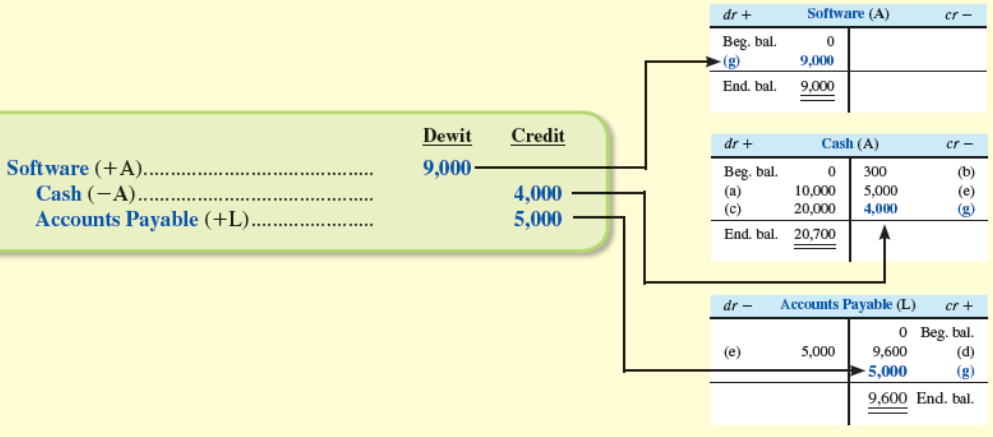
\includegraphics[width=1\columnwidth]{images/c2/post_entry.png}
		\caption{\label{fig:posting}\textbf{Posting to Ledger.} The debit to 
		Software in the 
		journal entry is copied into the debit (left) 
			side of its T-account. The credits to Cash and Accounts Payable are 
			copied 
			into the credit (right) side of those T-accounts.}	
	\end{figure}
	
	The simplified version 
	of a ledger account is called a T-account. Each T-account represents the 
	debit and credit columns of a ledger account. It also shows how an 
	individual journal entry’s effects would be summarized in these T-accounts. 
	Notice the following in Figure \ref{fig:posting}:
	\begin{itemize}[noitemsep]
		\item Every account starts with a beginning balance, normally on the 
		side where increases are summarized. For balance sheet accounts, the 
		ending balance from the prior period is the beginning balance for the 
		current period.
		\item Each amount is accompanied by a reference to the related journal 
		entry, which makes it easy to trace back to the original transaction 
		should errors occur.
		\item To calculate the ending balance in each account, you must start 
		with the beginning balance, add the amounts on the “+” side of the 
		T-account, and then subtract the amounts on the “-” side of the 
		T-account. The ending balance is double underlined to distinguish it 
		from transactions and symbolize the final result of a computation. The 
		ending balance is shown on the side that has the greater total dollar 
		amount.
	\end{itemize}
	
	\begin{figure}[ht!]
		\centering
		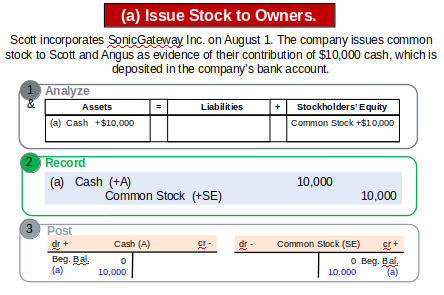
\includegraphics[width=1\columnwidth]{images/c2/records_eg1.png}
		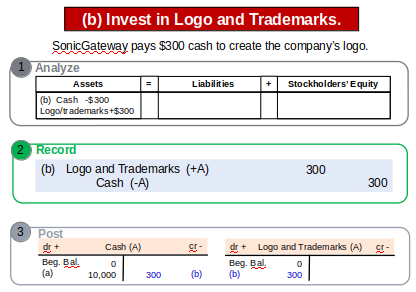
\includegraphics[width=1\columnwidth]{images/c2/records_eg2.png}
		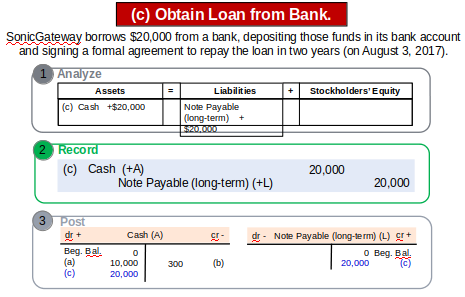
\includegraphics[width=1\columnwidth]{images/c2/records_eg3.png}
		\caption{Example of Accounting Process}
		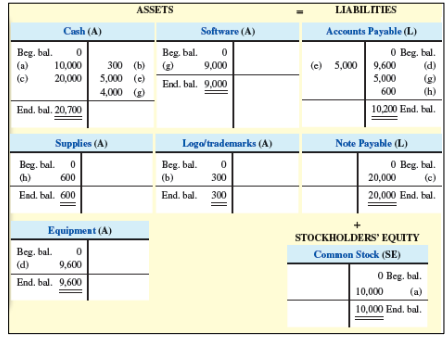
\includegraphics[width=1\columnwidth]{images/c2/t_accounts_eg.png}
		\caption{Example of T-Accounts}
	\end{figure}

	\subsection{Preparing Trial Balance}
	
	The next step in the accounting cycle is to prepare an internal accounting 
	report called a \textbf{trial balance} \ie Figure \ref{fig:trial_balance}. 
	It checks that the accounting 
	records are in balance by determining whether the sum of credits equate to 
	the sum of debits.The trial balance lists the ending balance in every 
	T-account and then computes total debits and total credits.
	
	\begin{figure}[ht]
		\centering
		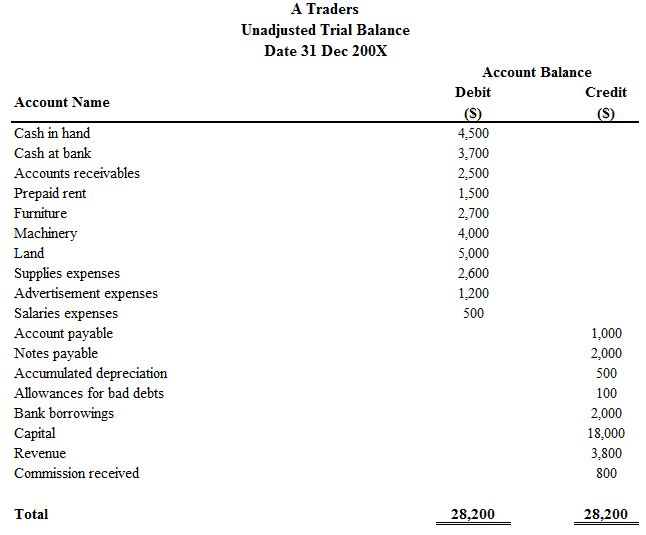
\includegraphics[width=1\columnwidth]{images/c2/How-to-Set-Up-a-Trial-Balance.jpg}
		\caption{Trial Balance}
		\label{fig:trial_balance}
	\end{figure}
	
	Preparing a trial balance involves three steps:
	\begin{enumerate}[noitemsep]
		\item List each account title and its amount (from ledger) in the trial 
		balance. If an account has zero balance, list it with a zero in its 
		normal balance column (or omit it entirely)
		\item Compute the total of debit balances and the total of credit 
		balances.
		\item Verify (prove) that total debit balance equal total credit 
		balances. 
	\end{enumerate}
	
	If the trial balance does not balance, the errors must be found and 
	corrected. An efficient way to search for an error is to check the 
	journalizing, posting and trial balance preparation in reverse order:
	\begin{enumerate}[noitemsep]
		\item Verify that the trial balance columns are correctly added.
		\item Verify that the account balances are accurately entered into the 
		ledger.
		\item See whether a debit or credit balance is mistakenly listed in the 
		trial balance as a credit or debit. 
		\item Recompute each account balance in the ledger. 
		\item Verify that each journal entry is appropriately posted. 
		\item Verify that the original journal entry has equal credits and 
		debits. 
	\end{enumerate}
	
	If an error is not discovered until after it is posted, we do not strike 
	through both erroneous entries in the journal and ledger. Instead, we 
	correct this error by creating a correcting entry that removes the amount 
	from the wrong account and record it to the correct account. 
	
	\subsection{Using Trial Balance to Prepare Financial Statements}
	
	After the trial balance has been prepared we begin preparing the financial 
	statements. We always begin with the income statement because net profit 
	appears on the statement of changes in equity. Next, we prepare the 
	statement of financial position and finally, we prepare the statement of 
	cash flows.
	
	\begin{figure}[ht]
		\centering
		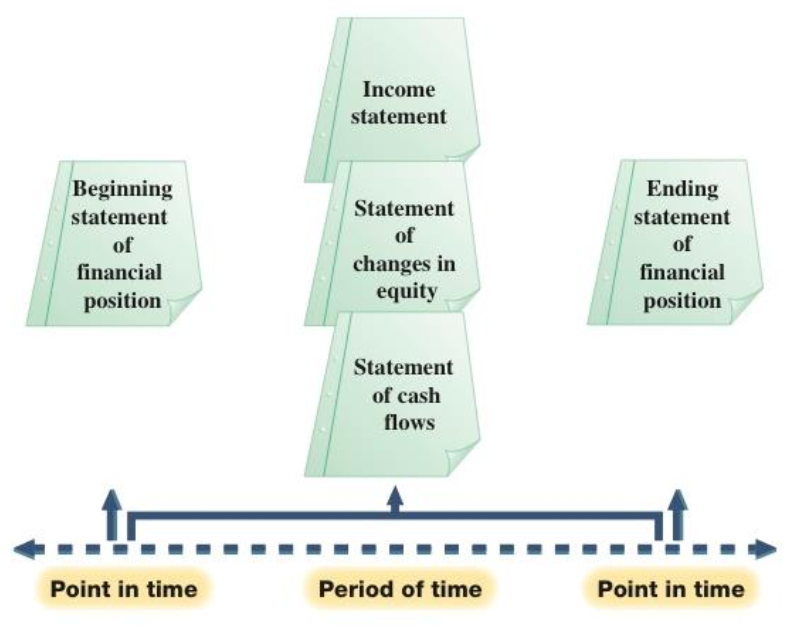
\includegraphics[width=1\columnwidth]{images/c2/preparing_financial_statements.png}
		\caption{Preparing Financial Statements}
	\end{figure}
	
	\subsection{Presentation Issues}
	
	Currency signs are usually not used in journals and ledgers. They do 
	often appear in financial statements and other documents such as trial 
	balances. 
	One practice is to put currency signs beside only the first and last 
	numbers in a column. It is also common to place the signs beside any key 
	amount that appears after a ruled line. 
	
	Some companies just state the currency in the report headings and do not 
	show currency signs for the column numbers. When amounts are entered in the 
	journal, ledger, or trial balance, commas are optional to indicate 
	thousands, millions, and so forth. Commas are always used in financial 
	statements. Companies commonly round amounts in reports to the nearest 
	dollar, or even to a higher level. 
	
\end{document}